\section{Results}\label{sec:results}

This section presents the experimental results and their implications for short-term prediction of Brazilian Mini-Index futures. Following the organization of the precursor, it first describes the common experimental setup and then discusses the performance of the individual model families. The expanded benchmark subsequently reports the direct cross-model comparison, exploratory statistical evidence, and economic outcomes.

\subsection{Experimental Setup and Data Partitioning}

All model--optimizer combinations use the seven descriptors described in Section~\ref{sec:featureselection}, the chronological split shown in Figure~\ref{fig:partition}, and the same 1,000-evaluation allowance per seed. RF, SVM, MLP, and 1D-CNN each are searched with RS, GA, PSO, DE, and GWO. The two protocols differ only in the validation fitness used to rank candidate configurations. Three common seeds (1--3) are available for every cell in both protocols.

Consequently, the direct comparison between fitness functions is descriptive: each reported model--optimizer result is the mean over the same three seeds. The locked test block contains 3,012 observations and is not used during search. This design differs from the randomized training and test sampling used in the precursor and removes look-ahead exposure from model selection.

\subsection{Reference Baselines}

Two deterministic reference models were evaluated on the same locked test block before interpreting the optimizer benchmark. The majority-direction baseline predicts the class that is more frequent in the training partition; its probability is fixed at that training prevalence. The default RF baseline uses the same fixed seven-feature representation and the final-refit rule (training plus validation), but no hyperparameter search. These references are not additional optimizers and do not enter the matched optimizer--seed statistical tests.

Table~\ref{tab:reference_baselines} illustrates why accuracy or positive-class $F_1$ alone are insufficient in this setting. The naive baseline predicts every test observation as an uptrend, obtaining $F_1=0.675$ because the positive class is common, but MCC is exactly zero. The default RF yields MCC 0.210 and balanced accuracy 0.604, establishing a temporal no-tuning reference. The optimized model summaries reported below must therefore be read as evidence beyond both a trivial directional rule and this default classifier, while acknowledging that the default RF is only one backbone-specific reference.

\begin{table}[htbp]
\centering
\caption{Locked-test reference baselines under the temporal protocol. The naive baseline selects the training-majority direction (uptrend); the default RF is refitted on training plus validation with 100 trees and no hyperparameter search.}
\label{tab:reference_baselines}
\footnotesize
\begin{tabular}{lrrrrr}\toprule
\textbf{Reference} & \textbf{Accuracy} & \textbf{Balanced accuracy} & \textbf{$F_1$} & \textbf{MCC} & \textbf{AUC-ROC}\\\midrule
Naive majority direction & 0.510 & 0.500 & 0.675 & 0.000 & 0.500\\
Default RF (no tuning) & 0.605 & 0.604 & 0.630 & 0.210 & 0.645\\\bottomrule
\end{tabular}
\end{table}

\subsection{Performance of the Models}
\label{sec:performance_models}

Table~\ref{tab:all_hyperparameters} retains the presentation pattern of the precursor: it states the search space and an illustrative GA-selected configuration for each of the four model families. The configurations are from seed 1 under Protocol A and are included to make the optimization procedure concrete; they are not asserted to be universally optimal because all optimizer--seed outcomes are summarized below.

\begin{sidewaystable}[htbp]
\centering
\caption{Hyperparameter search domains and representative GA-selected configurations across the four evaluated classifier backbones.}
\label{tab:all_hyperparameters}
\small
\begin{tabular}{lllclll}\toprule
\multicolumn{3}{c}{\textbf{Random Forest (RF)}} & & \multicolumn{3}{c}{\textbf{Support Vector Machine (SVM)}} \\\cmidrule{1-3}\cmidrule{5-7}
\textbf{Hyperparameter} & \textbf{Search space} & \textbf{Selected} & & \textbf{Hyperparameter} & \textbf{Search space} & \textbf{Selected}\\\midrule
$n_{\mathrm{estimators}}$ & $[50,500]$ & 58 & & $C$ & $[10^{-3},10^{3}]$ (log scale) & 2.089\\
$\mathrm{max\_depth}$ & $[5,50]$ & 6 & & $\gamma$ & $[10^{-5},10^{1}]$ (log scale) & 5.044\\
$\mathrm{min\_samples\_split}$ & $[2,20]$ & 13 & & Kernel & $\{\mathrm{linear},\mathrm{RBF}\}$ & linear\\
$\mathrm{min\_samples\_leaf}$ & $[1,20]$ & 15 & & & & \\
$\mathrm{max\_features}$ & $\{\mathrm{sqrt},\mathrm{log2},\mathrm{None}\}$ & None & & & & \\
$\mathrm{class\_weight}$ & $\{\mathrm{None},\mathrm{balanced}\}$ & None & & & & \\\midrule
\multicolumn{3}{c}{\textbf{Multilayer Perceptron (MLP)}} & & \multicolumn{3}{c}{\textbf{1D Convolutional Neural Network (1D-CNN)}} \\\cmidrule{1-3}\cmidrule{5-7}
\textbf{Hyperparameter} & \textbf{Search space} & \textbf{Selected} & & \textbf{Hyperparameter} & \textbf{Search space} & \textbf{Selected}\\\midrule
Hidden neurons & $[5,500]$ & 410 & & Filters & $[8,128]$ & 48\\
Learning rate & $[10^{-8},10^{-2}]$ (log scale) & $3.42\times10^{-4}$ & & Kernel size & $[2,5]$ & 3\\
$L_2$ regularization & $[10^{-8},10^{-2}]$ (log scale) & $1.66\times10^{-7}$ & & Dense neurons & $[16,256]$ & 251\\
Dropout rate & $[0,0.10]$ & 0.057 & & Learning rate & $[10^{-8},10^{-2}]$ (log scale) & $3.90\times10^{-6}$\\
Batch size & $\{16,32,64,80,112,128\}$ & 112 & & $L_2$ regularization & $[10^{-8},10^{-2}]$ (log scale) & $5.70\times10^{-6}$\\
& & & & Dropout rate & $[0,0.10]$ & 0.026\\
& & & & Batch size & $\{16,32,64,80,112,128\}$ & 16\\\bottomrule
\end{tabular}
\end{sidewaystable}

Figures~\ref{fig:rf_convergence}--\ref{fig:cnn_convergence} replace the three GA-only convergence plots of the precursor with the five budget-matched search trajectories. For each model, the left panel follows the compound MCC/$F_1$ fitness and the right panel follows weighted training/validation accuracy. The vertical scales differ because the objectives differ; their role is to show search convergence within a protocol, not to compare objective magnitudes across protocols.

\begin{figure}[htbp]\centering
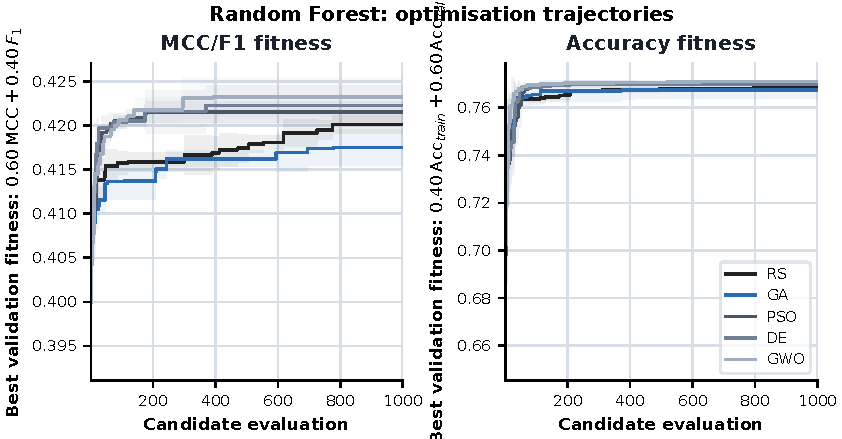
\includegraphics[width=0.93\linewidth]{figures/ijcnn_style_rf_convergence.pdf}
\caption{Fitness evolution during equal-budget optimization of the Random Forest model. Lines summarize the three common seeds.}
\label{fig:rf_convergence}\end{figure}

\begin{figure}[htbp]\centering
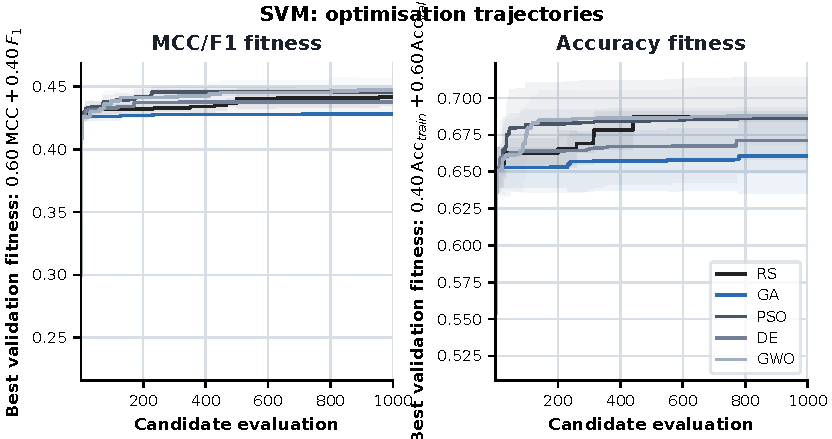
\includegraphics[width=0.93\linewidth]{figures/ijcnn_style_svm_convergence.pdf}
\caption{Fitness evolution during equal-budget optimization of the SVM model. Lines summarize the three common seeds.}
\label{fig:svm_convergence}\end{figure}

\begin{figure}[htbp]\centering
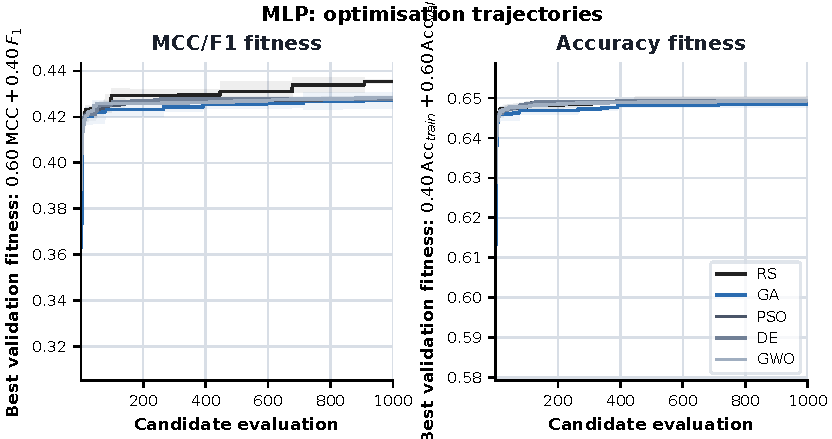
\includegraphics[width=0.93\linewidth]{figures/ijcnn_style_mlp_convergence.pdf}
\caption{Fitness evolution during equal-budget optimization of the MLP model. Lines summarize the three common seeds.}
\label{fig:mlp_convergence}\end{figure}

\begin{figure}[htbp]\centering
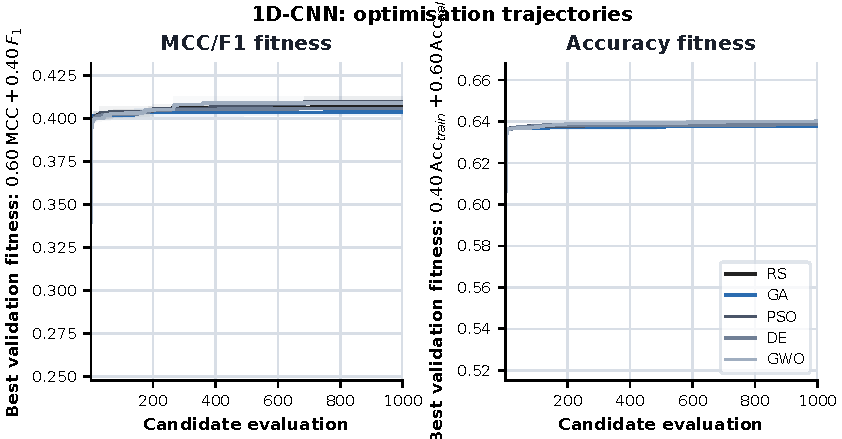
\includegraphics[width=0.93\linewidth]{figures/ijcnn_style_cnn_convergence.pdf}
\caption{Fitness evolution during equal-budget optimization of the 1D-CNN model. Lines summarize the three common seeds.}
\label{fig:cnn_convergence}\end{figure}

\subsection{Optimizer-Level Performance Under Equal Budget}

Table~\ref{tab:optimizer_primary_metrics} exposes the comparison that is obscured when results are first aggregated across optimizers. Every cell is the mean locked-test primary metric across the same three seeds, and every optimizer consumed the same 1,000 candidate evaluations. The table is descriptive rather than inferential: it establishes the observed optimizer-by-backbone pattern, while the small number of seeds prevents a reliable universal ranking of optimizers.

Under MCC/$F_1$ fitness, GA, PSO, and DE reach similarly high mean MCC values for RF, whereas the MLP rows favour the population methods over Random Search. The pattern is less uniform for SVM and 1D-CNN, for which the ordering changes with the optimizer. Under weighted-accuracy fitness, MLP remains close to 0.65 accuracy for all five methods, while RF and SVM are more sensitive to the optimizer choice. These contrasts motivate the model-level aggregation in the next subsection, but they also show why an optimizer cannot be declared superior from one pooled summary.

\begin{table}[htbp]
\centering
\caption{Optimizer-level locked-test primary metrics under equal budget. Each cell is a mean over three common seeds; boldface denotes the largest mean within a model and protocol. RS: Random Search; GA: Genetic Algorithm; PSO: Particle Swarm Optimization; DE: Differential Evolution; GWO: Grey Wolf Optimizer.}
\label{tab:optimizer_primary_metrics}
\footnotesize
\begin{tabular}{lccccc}\toprule
\textbf{Model} & \textbf{RS} & \textbf{GA} & \textbf{PSO} & \textbf{DE} & \textbf{GWO}\\\midrule
\multicolumn{6}{c}{\textbf{Panel A: MCC/$F_1$ fitness; locked-test MCC}}\\\midrule
RF & 0.281 & \textbf{0.293} & 0.293 & 0.292 & 0.288\\
SVM & 0.105 & \textbf{0.290} & 0.255 & 0.187 & 0.232\\
MLP & 0.106 & 0.290 & 0.299 & 0.302 & \textbf{0.305}\\
1D-CNN & 0.179 & 0.268 & \textbf{0.269} & 0.267 & 0.139\\\midrule
\multicolumn{6}{c}{\textbf{Panel B: weighted-accuracy fitness; locked-test accuracy}}\\\midrule
RF & 0.604 & \textbf{0.611} & 0.604 & 0.600 & 0.602\\
SVM & 0.588 & 0.557 & 0.571 & 0.584 & \textbf{0.593}\\
MLP & 0.649 & 0.649 & \textbf{0.652} & 0.652 & 0.652\\
1D-CNN & 0.636 & 0.634 & 0.635 & 0.634 & \textbf{0.637}\\\bottomrule
\end{tabular}
\end{table}

\subsection{Model-Level Aggregation Across Optimizers}

Table~\ref{tab:predictive_summary} and Figure~\ref{fig:model_comparison} present locked-test performance aggregated over 15 optimizer--seed blocks per model within each protocol. Reporting the standard deviation is essential here: the blocks combine five optimizers and three common seeds, so the dispersion describes sensitivity to the evaluated search procedure rather than independent market replications. Under MCC/$F_1$ fitness, RF has the largest mean test accuracy (0.645), MCC (0.289), and $F_1$ (0.664), with markedly lower variability than the other backbones. Under weighted-accuracy fitness, MLP has the largest mean accuracy (0.651), MCC (0.301), and $F_1$ (0.658). Thus, the validation objective changes the descriptive ordering of the model families and should not be treated as interchangeable with the final reporting metric.

\begin{table}[htbp]
\centering
\caption{Locked-test predictive outcomes by backbone and validation protocol. Entries are mean $\pm$ standard deviation over 15 optimizer--seed blocks per row (five optimizers $\times$ three common seeds).}
\label{tab:predictive_summary}
\small
\begin{tabular}{lccc|ccc}\toprule
& \multicolumn{3}{c|}{\textbf{MCC/$F_1$ fitness}} & \multicolumn{3}{c}{\textbf{Weighted accuracy fitness}}\\
\textbf{Model} & Accuracy & MCC & $F_1$ & Accuracy & MCC & $F_1$\\\midrule
RF & $0.645\pm0.004$ & $0.289\pm0.008$ & $0.664\pm0.006$ & $0.604\pm0.005$ & $0.208\pm0.009$ & $0.624\pm0.004$\\
SVM & $0.604\pm0.060$ & $0.214\pm0.132$ & $0.602\pm0.122$ & $0.578\pm0.028$ & $0.159\pm0.053$ & $0.600\pm0.071$\\
MLP & $0.630\pm0.070$ & $0.261\pm0.141$ & $0.639\pm0.071$ & $0.651\pm0.003$ & $0.301\pm0.005$ & $0.658\pm0.004$\\
1D-CNN & $0.613\pm0.056$ & $0.224\pm0.120$ & $0.597\pm0.166$ & $0.635\pm0.002$ & $0.271\pm0.005$ & $0.639\pm0.007$\\\bottomrule
\end{tabular}
\end{table}

\begin{figure}[htbp]\centering
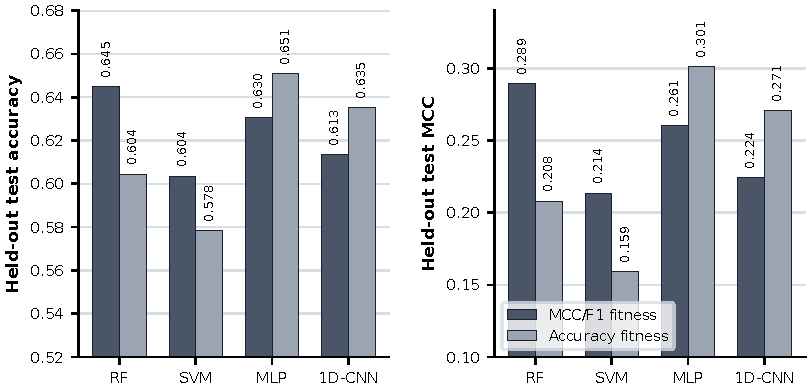
\includegraphics[width=0.94\linewidth]{figures/ijcnn_style_model_performance.pdf}
\caption{Comparison of mean locked-test accuracy and MCC for all four model families under the two validation objectives.}
\label{fig:model_comparison}\end{figure}

\subsection{Exploratory Statistical Evidence}

The model-level tests are performed separately within each holdout protocol. The five optimizer--seed combinations yield 15 matched blocks for each backbone. Table~\ref{tab:predictive_inference} reports the two preselected endpoint tests that correspond to the respective validation objectives. Under MCC/$F_1$ fitness, the Friedman comparison of locked-test MCC is significant ($\chi^2=22.84$, $p=4.36\times10^{-5}$). RF has the largest marginal mean MCC (Table~\ref{tab:predictive_summary}), whereas MLP has the best mean rank across the matched blocks; this distinction is precisely why both summaries are reported. Under weighted-accuracy fitness, the accuracy comparison is significant ($\chi^2=42.92$, $p=2.56\times10^{-9}$), and MLP is first both by mean accuracy and mean rank. Its Holm-adjusted contrasts against RF, SVM, and 1D-CNN are all significant ($p_{\mathrm{Holm}}\approx0.00194$).

\begin{table}[htbp]
\centering
\caption{Exploratory Friedman tests for the endpoint aligned with each validation protocol. Lower mean rank is better. The blocks are optimizer--seed combinations from one locked chronological segment and are not independent market replications.}
\label{tab:predictive_inference}
\small
\begin{tabular}{llrrrrrrrr}\toprule
\textbf{Protocol} & \textbf{Endpoint} & $n$ & $\chi^2$ & $p$ & RF & SVM & MLP & 1D-CNN\\
& & & & & \multicolumn{4}{c}{\textbf{Mean rank}}\\\midrule
MCC/$F_1$ fitness & Test MCC & 15 & 22.84 & $4.36\times10^{-5}$ & 2.07 & 2.73 & 1.53 & 3.67\\
Weighted accuracy fitness & Test accuracy & 15 & 42.92 & $2.56\times10^{-9}$ & 3.13 & 3.87 & 1.00 & 2.00\\\bottomrule
\end{tabular}
\end{table}

Because these blocks share one chronological test segment and only three random seeds, the tests summarize variation across the evaluated optimizer--seed combinations. They do not establish independent replication across market periods, nor do they test a confirmatory difference between the two fitness functions. The inferential results should therefore be read together with the descriptive dispersion in Table~\ref{tab:predictive_summary}, rather than as a claim that one backbone is universally superior.

\subsection{Exploratory Economic Evaluation}

The economic evaluation yields a complementary ranking under the fixed intrabar execution rule. Table~\ref{tab:economic_summary} reports the complete set of economic endpoints rather than total profit alone. Under MCC/$F_1$ fitness, RF has the largest mean total profit (26,465 points), the highest mean profit factor, and the smallest drawdown dispersion. Under weighted-accuracy fitness, MLP has the largest mean total profit (27,737 points) and profit factor, whereas RF has the least negative mean maximum drawdown (-1,866 points). Thus, the predictive winner and the return--risk profile do not always coincide. Figure~\ref{fig:economic_comparison} visualizes the profit--drawdown component of this comparison; it should not be read as a transaction-cost-complete trading recommendation.

\begin{table}[htbp]
\centering
\caption{Exploratory economic outcomes under the fixed intrabar execution rule. Net profit and maximum drawdown (Max. DD) are points; PF denotes profit factor and Sharpe is annualized. Entries are mean $\pm$ standard deviation over 15 optimizer--seed blocks.}
\label{tab:economic_summary}
\footnotesize
\begin{tabular}{llrrrr}\toprule
\textbf{Protocol} & \textbf{Model} & \textbf{Net profit} & \textbf{Max. DD} & \textbf{PF} & \textbf{Sharpe}\\\midrule
\multirow{4}{*}{MCC/$F_1$ fitness} & RF & $26{,}465\pm1{,}732$ & $-2{,}126\pm141$ & 1.48 & 12.50\\
& SVM & $17{,}017\pm29{,}437$ & $-9{,}823\pm17{,}123$ & 1.39 & 8.52\\
& MLP & $22{,}110\pm20{,}556$ & $-5{,}503\pm12{,}984$ & 1.43 & 10.62\\
& 1D-CNN & $19{,}969\pm17{,}574$ & $-5{,}991\pm10{,}469$ & 1.37 & 7.67\\\midrule
\multirow{4}{*}{Weighted accuracy fitness} & RF & $21{,}973\pm1{,}336$ & $-1{,}866\pm365$ & 1.38 & 11.95\\
& SVM & $11{,}440\pm13{,}350$ & $-5{,}241\pm1{,}961$ & 1.21 & 4.18\\
& MLP & $27{,}737\pm1{,}069$ & $-2{,}141\pm112$ & 1.51 & 13.07\\
& 1D-CNN & $26{,}861\pm1{,}924$ & $-2{,}494\pm62$ & 1.49 & 9.71\\\bottomrule
\end{tabular}
\end{table}

\begin{figure}[htbp]\centering
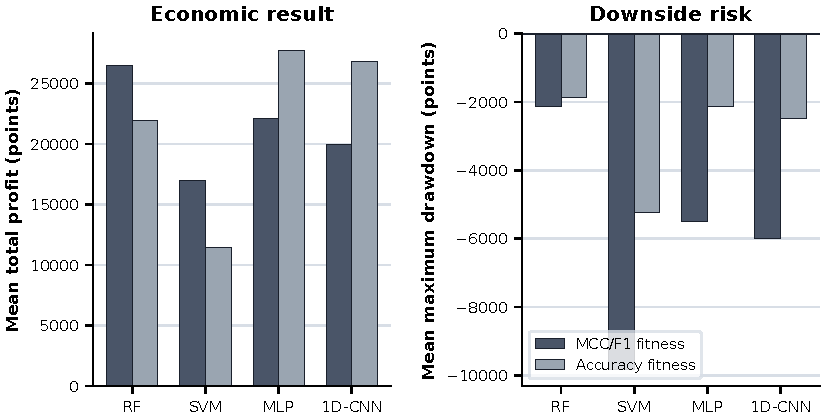
\includegraphics[width=0.94\linewidth]{figures/ijcnn_style_economic_summary.pdf}
\caption{Mean total profit and maximum drawdown across 15 optimizer--seed blocks per model. Results are reported separately for the two validation objectives.}
\label{fig:economic_comparison}\end{figure}
